\documentclass[a4paper, 10pt]{article}
\usepackage{amsmath}
\usepackage{graphicx}
\title{Project 1 - INF5620}
\author{Henrik Andersen Sveinsson}


\begin{document}
\maketitle

%%%%%%%%%%%%%%%%%%%%%%%%%%%%%%%%%%%%%%%%%%%%%%%%%%%%%%%%
\section{Setting up the differential equation}
Beginning with newtons second law for an object falling  with quadratic  air resistance and a source term for verification.
\begin{equation}
	\sum F = m\ddot{x}
\end{equation}

% note to self: What is a source term, which is given in the exercise

\begin{equation}
	mg - b\dot{x}|\dot{x}| + F_s = m\ddot{x}
\end{equation}
Or, written in terms of velocity.
\begin{equation}
	mg- bv|v| + F_s = m\dot{v}
\end{equation}
\begin{equation}
	\dot{v} = g - \frac{b}{m}v|v| + F_s = f(t, v)
\end{equation}

%%%%%%%%%%%%%%%%%%%%%%%%%%%%%%%%%%%%%%%%%%%%%%%%%%%%%%%
\section{Setting up the discrete equation}
\label{sec:setting_up_the_discrete_equation}

We choose the Crank-Nicholson scheme for discretizing the equation. 
\begin{equation}
	[D_t v = f(t, \bar{v}^{t, \frac{1}{2}})]^{n+\frac{1}{2}}
\end{equation}
To linearize the equation, we decide to take the geometric average of the velocities in $|v|v$, such that:
\begin{equation}
	\frac{v^{n+1} - v^{n}}{\Delta t} = g - \frac{b}{m}|v^n|v^{n+1} + F_s
\end{equation}
This gives a linear equation in $v^{n+1}$, which makes it easier to handle with an implicit solver. Solving this equation for $v^{n+1}$ gives:
\begin{equation}
	v^{n+1} = \frac{v^n + (g +F_s)\Delta t}{1+\frac{b}{m}|v^n|\Delta t}
\end{equation}

Checking whether a linear solution will solve the discrete equation without the source term. I do this by inserting the solution $v(t) = t$, and solving for $F_s$.  
\begin{equation}
	\left[D_t t = g - \frac{b}{m} |t_n|t_{n+1} + F_s\right]^{n+\frac{1}{2}}
\end{equation}
\begin{equation}
	F_s = \frac{b}{m} t(t+\Delta t) - g + 1 
\end{equation}

With this source term, $v(t) = t$ is the exact soultion to the discrete equation. Inserting this source term into the solver should give a solution that holds up to machine precision. This holds, and a nose test with a tolerance of $1e-13$ is implemented.

\section{Improved force expression for parachuter}
A simple force model for a parachuter at high reynolds numbers is the following.
\begin{equation}
	F(t, v) = F_d^{(q)} + F_g + F_b
\end{equation}
The quadratic drag expression is chosen to be $-\frac{1}{2}C_D \rho A |v|v$, where $C_D$ is a dimensionless drag coefficient and $A$ is the cross sectional area of the falling body. $\rho$ is the air density. The gravitational pull is taken as the constant $mg$, implying that we are close to the surface of the earth. We assume constant air density, so the bouyancy term is $\rho g V$, where $V$ is the volume of the body. 

Applying Newtons 2. law, gives:
\begin{equation}
	m\dot{v}(t, v) = -\frac{1}{2}C_D \rho A |v|v + mg - \rho g V
\end{equation}
The positgive direction of motion is towards ground.
Now, a few manipulations to get the equation more suited for numerical treatment:
We introduce the density $\rho_b$ of the falling body, so that $m = \rho_b V$. Dividing by the mass, ans inserting $\rho_b V$ gives:
\begin{equation}
	\dot{v}(t, v) = -\frac{1}{2} C_D \frac{\rho A}{\rho_b V}|v|v + g\left( 1- \frac{\rho}{\rho_b} \right) 
\end{equation}
We now define 
$a = \frac{1}{2} C_D \frac{\rho A}{\rho_b V}$ 
and 
$b = g\left( 1- \frac{\rho}{\rho_b}\right)$, 
such that the equation to solve numerically is:

\begin{equation}
	\dot{v}(t, v) = -a|v|v + b + f_s(t)
\end{equation}

Where we have added a source term $f_s(t)$ to be able to manufacture solutions.

Applying the Crank-Nicolson scheme on this equation:

\begin{equation}
	\left[ D_t v = f(t, \bar{v}^{t, \frac{1}{2}})\right]^{n+\frac{1}{2}}
\end{equation}
Written out, with $[|v|v]^{n+\frac{1}{2}} \approx |v^{n}|v^{n+1}$
\begin{equation}
	\frac{v^{n+1}-v^{n}}{\Delta t} = -a |v^{n}| v^{n+1} + b + f_s(t_{n+\frac{1}{2}})
\end{equation}
Where the source term is supposed to be defined later, and we assume it to be evaluable at $t_{n+\frac{1}{2}}$.

\begin{equation}
	v^{n+1} = \frac{v^n + (b + f_s(t))\Delta t }{1 + a |v^n| \Delta t}.
\end{equation}

We now manufacture a linear solution to the problem, $v(t) = At+B$, Where the initial state $v(0) = B$. Inserted into the CN-scheme, this gives:
\begin{equation}
	A = -a|At+B|(A(t+\Delta t) + B) + b+ f_s(t_{n+\frac{1}{2}})
\end{equation}
Which gives:
\begin{equation}
	f_s(t_{n+\frac{1}{2}}) = a|At+B|(A(t+\Delta t) + B) - b + A
\end{equation}
A test for this manufactured solution is made.

To check the convergence rate, we construct a solution to the continous problem, still on the form $At+ B$.
\begin{equation}
	D[At+B] = -a|At+B|(At+B) + b + f_s(t)
\end{equation}
Such that:
\begin{equation}
	f_s(t) = a|At+B|(At+B) - b + A
\end{equation}

Using this source term, the convergence is confirmed to be quadratic.
\begin{figure}
\centering
	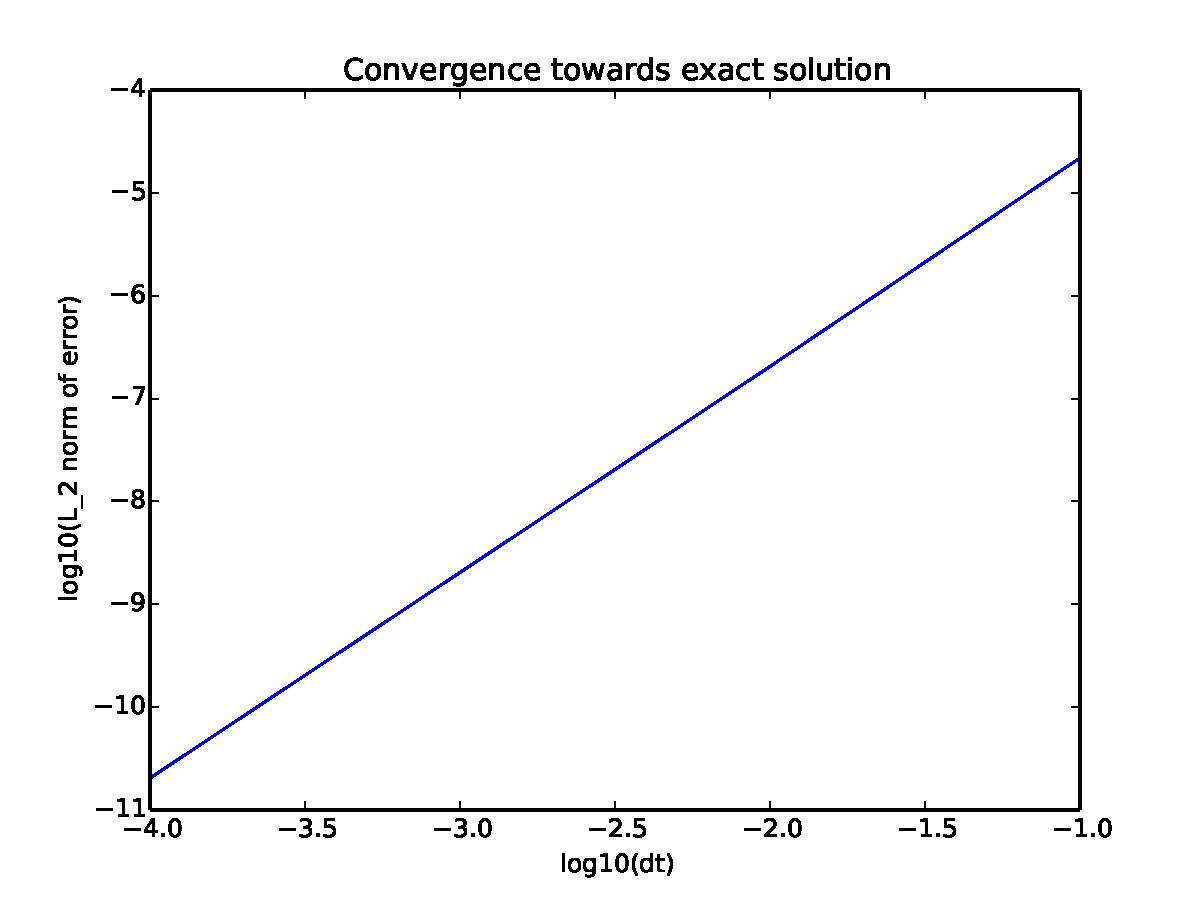
\includegraphics[width=0.8\textwidth]{figures/convergence.pdf}
	\caption{Error estimate shows second order convergence in $\Delta t$}
\end{figure}


\end{document}